\documentclass[11pt,a4paper,twoside]{article}

\usepackage[utf8]{inputenc}
\usepackage[T1]{fontenc}
\usepackage[ngerman]{babel}
\usepackage{lmodern}
\usepackage{amsmath,amssymb}
\usepackage{graphicx}
\usepackage{booktabs,tabularx,array}
\usepackage[table]{xcolor}
\usepackage{tikz}
\usetikzlibrary{arrows.meta,positioning,shapes.geometric,calc}
\usepackage[most]{tcolorbox}
\usepackage{enumitem}
\usepackage{microtype}
\usepackage{fancyhdr}
\usepackage{hyperref}
\usepackage[a4paper,left=18mm,right=18mm,top=18mm,bottom=19mm,headheight=14pt]{geometry}

\definecolor{navy}{HTML}{174A63}
\definecolor{blue}{HTML}{2E7698}
\definecolor{lightblue}{HTML}{EAF3F7}
\definecolor{lightgray}{HTML}{F2F3F4}
\definecolor{midgray}{HTML}{66727A}
\definecolor{green}{HTML}{477A63}
\definecolor{orange}{HTML}{B96A2B}

\hypersetup{colorlinks=true,linkcolor=navy,urlcolor=blue,pdftitle={Entscheidungsbäume -- kompakte Schülerversion}}
\setlength{\parindent}{0pt}
\setlength{\parskip}{4pt}
\setlist[itemize]{leftmargin=5mm,itemsep=1.5pt,topsep=2pt}
\setlist[enumerate]{leftmargin=6mm,itemsep=2pt,topsep=2pt}
\renewcommand{\familydefault}{\sfdefault}

\pagestyle{fancy}
\fancyhf{}
\fancyhead{}
\fancyfoot[C]{\small\thepage}
\renewcommand{\headrulewidth}{0pt}

\newtcolorbox{definition}[1][]{enhanced,breakable,colback=lightblue,colframe=blue,
  boxrule=0.8pt,arc=1.5mm,left=3mm,right=3mm,top=2mm,bottom=2mm,
  fonttitle=\bfseries,title=Definition,#1}
\newtcolorbox{merke}[1][]{enhanced,breakable,colback=lightgray,colframe=navy,
  boxrule=0.9pt,arc=1.5mm,left=3mm,right=3mm,top=2mm,bottom=2mm,
  fonttitle=\bfseries,title=Merke,#1}
\newtcolorbox{beispiel}[1][]{enhanced,breakable,colback=white,colframe=midgray,
  boxrule=0.7pt,arc=1.5mm,left=3mm,right=3mm,top=2mm,bottom=2mm,
  fonttitle=\bfseries,title=Beispiel,#1}
\newtcolorbox{ueberblick}[1][]{enhanced,breakable,colback=lightblue,colframe=navy,
  boxrule=1.1pt,arc=1.5mm,left=3mm,right=3mm,top=2.5mm,bottom=2.5mm,
  fonttitle=\bfseries,title=Überblick,#1}

\newcommand{\fach}[1]{\textbf{\color{navy}#1}}
\newcommand{\sectionline}[1]{%
  \vspace{1mm}{\Large\bfseries\color{navy}#1}\par\vspace{1mm}%
  {\color{blue}\rule{\linewidth}{0.8pt}}\vspace{1mm}}
\newcommand{\subline}[1]{\vspace{1mm}{\large\bfseries\color{navy}#1}\par}

\begin{document}

% Seite 1
\begin{tcolorbox}[colback=navy,colframe=navy,arc=2mm,boxrule=0pt,left=5mm,right=5mm,top=4mm,bottom=4mm]
  {\color{white}\fontsize{24}{28}\selectfont\bfseries Entscheidungsbäume}\par
  \vspace{1mm}{\color{white}\large Kompaktes Lern- und Nachschlageheft · Informatik 11}
\end{tcolorbox}

\sectionline{1. Entscheidungsbäume}

Ein \fach{Entscheidungsbaum} ist ein Modell zur \fach{Klassifikation}: Er ordnet neue Daten anhand ihrer
Merkmale einer Klasse zu. Entscheidungsbäume können durch \fach{überwachtes Lernen} aus Beispielen mit
bekanntem Ergebnis erzeugt werden. Sie werden immer von unten nach oben durchlaufen.

\begin{definition}[title=Definition: Überwachtes Lernen]
Beim \fach{überwachten Lernen} wird aus \fach{gelabelten Daten} ein Modell erzeugt. Gelabelte Daten besitzen
neben ihren Merkmalen ein bekanntes \fach{Label}, also die richtige Klasse. Das Lernverfahren sucht Regeln,
mit denen es anschließend neue Eingaben klassifizieren kann.
\end{definition}

\begin{center}
  
\includegraphics[width=0.76\linewidth]{images/ueberwachtes-lernen.png}

  {\scriptsize\color{midgray}Abbildung: Stefan Seegerer, Tilman Michaeli und Sven Jatzlau, CC BY; übernommen aus dem Ausgangsmaterial.}
\end{center}

\sectionline{2. Aufbau eines Entscheidungsbaums}

\begingroup\small
\begin{center}
\begin{tikzpicture}[scale=0.82,transform shape,>=Latex,font=\small,every node/.style={align=center},
  decision/.style={draw=navy,fill=lightblue,rounded corners=1mm,minimum width=27mm,minimum height=9mm},
  leaf/.style={draw=midgray,fill=lightgray,rounded corners=1mm,minimum width=21mm,minimum height=9mm}]
  \node[decision] (root) at (0,0) {Mundform?};
  \node[leaf] (teeth) at (-6.3,-2.2) {beißt nicht};
  \node[leaf] (tongue) at (-2.7,-2.2) {beißt nicht};
  \node[decision] (openmouth) at (0.7,-2.2) {Augen als X?};
  \node[decision] (closedmouth) at (6.0,-2.2) {beide Augen\\offen?};
  \node[leaf] (openyes) at (-0.8,-4.4) {beißt};
  \node[leaf] (openno) at (2.2,-4.4) {beißt nicht};
  \node[leaf] (closedyes) at (4.5,-4.4) {beißt nicht};
  \node[leaf] (closedno) at (7.5,-4.4) {beißt};
  \draw (root) -- node[above left,font=\footnotesize]{Zähne} (teeth);
  \draw (root) -- node[above left,font=\footnotesize]{Zunge} (tongue);
  \draw (root) -- node[above right,font=\footnotesize]{offen} (openmouth);
  \draw (root) -- node[above right,font=\footnotesize]{geschlossen} (closedmouth);
  \draw (openmouth) -- node[above left,font=\footnotesize]{ja} (openyes);
  \draw (openmouth) -- node[above right,font=\footnotesize]{nein} (openno);
  \draw (closedmouth) -- node[above left,font=\footnotesize]{ja} (closedyes);
  \draw (closedmouth) -- node[above right,font=\footnotesize]{nein} (closedno);
\end{tikzpicture}
\end{center}

\begin{itemize}
  \item Ein \fach{Entscheidungsknoten} prüft ein Attribut.
  \item Eine \fach{Kante} steht für eine Merkmalsausprägung und führt zum nächsten Knoten.
  \item Ein \fach{Blatt} enthält die vorhergesagte Klasse bzw. das Label.
\end{itemize}

\begin{beispiel}[title=Beispiel: eine Vorhersage]
Ein Äffchen mit \emph{Mundform = offen} und \emph{Augenstellung = X} folgt im obigen Baum zweimal der
passenden Kante. Es erreicht das Blatt \emph{beißt}; dies ist die Vorhersage des Modells.
\end{beispiel}
\endgroup

\newpage\thispagestyle{fancy}

\sectionline{3. Trainings- und Testdaten}

Die verfügbaren gelabelten Daten werden getrennt verwendet:

\begin{itemize}
  \item \fach{Trainingsdaten} sind gelabelt bzw. beschriftet und werden zur Erzeugung des Modells verwendet.
  \item \fach{Testdaten} sind gelabelt bzw. beschriftet und werden zur Beurteilung der Vorhersagequalität verwendet.
\end{itemize}

\begin{beispiel}[title=Beispiel: gelabelte Trainingsdaten]
Die bekannten Äffchen sind mit den Labels \emph{beißt} oder \emph{beißt nicht} versehen. Aus diesen
Beispielen kann ein Entscheidungsbaum Regeln für die Klassifikation neuer Äffchen lernen.

\begin{center}
  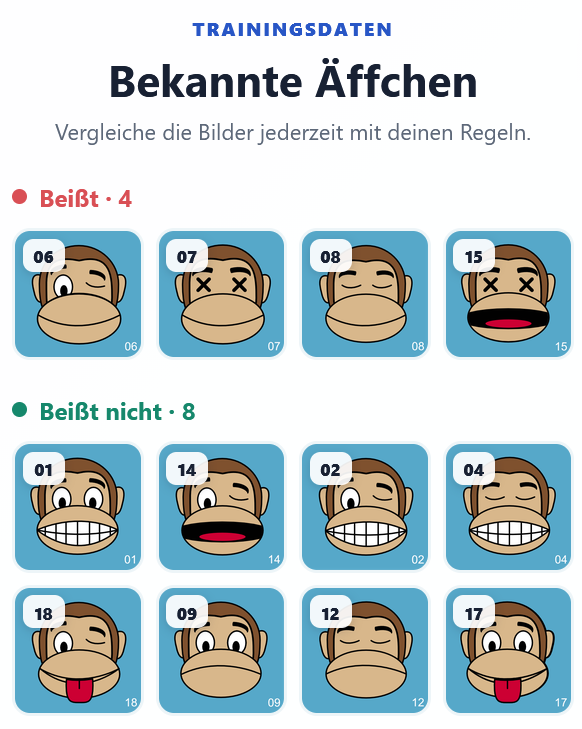
\includegraphics[width=0.52\linewidth]{images/trainingsdaten-bekannte-aeffchen.png}

  {\scriptsize\color{midgray}Beispielgrafik: vom Nutzer bereitgestellt; Äffchen-Illustrationen im Ausgangsmaterial von Annabel Lindner und Stefan Seegerer, CC BY-NC.}
\end{center}
\end{beispiel}

\begin{merke}
Die Trennung verhindert, dass ein Modell nur an bereits bekannten Daten gut wirkt. Erst neue Testdaten zeigen,
wie zuverlässig seine \fach{Vorhersagen} sind. \\
Zwei Entscheidungsbäume können dieselben Trainingsdaten vollständig richtig klassifizieren und bei unbekannten
Testdaten trotzdem unterschiedlich gut funktionieren. \\ Die Trainingsdaten müssen nicht jede mögliche
Merkmalskombination enthalten.
\end{merke}

\newpage\thispagestyle{fancy}

% Seite 3
\sectionline{4. Fehlklassifikation und Informationsgewinn}

Ein Entscheidungsbaum wird aus gelabelten Trainingsdaten aufgebaut. Im Beispiel sind es 9 Fische mit den
Attributen \emph{Schuppenfarbe}, \emph{Muster}, \emph{Bauchfarbe} und \emph{Flossenfarbe} sowie dem Label
\emph{friedlich} oder \emph{feindselig}.

\begin{definition}[title=Definition: Fehlklassifikation und Informationsgewinn]
Ein Knoten sagt für seine Teilmenge das häufigere Label voraus. Alle Daten mit dem anderen Label sind
\fach{Fehlklassifikationen}. Der \fach{Informationsgewinn} eines Splits ist
\[
  IG=\text{Fehler vor dem Aufteilen}-\text{Gesamtfehler nach dem Aufteilen}.
\]
Gewählt wird das Attribut mit dem größten Informationsgewinn.
\end{definition}

\begin{beispiel}[title=Beispiel: erster Split der 9 Trainingsfische]
Ohne Split: 4 friedlich, 5 feindselig. Der Baum sagt \emph{feindselig} voraus; es entstehen 4 Fehler.

\smallskip
\begin{minipage}[t]{0.61\linewidth}
\vspace{0pt}
\renewcommand{\arraystretch}{1.1}\setlength{\tabcolsep}{4pt}
\begin{tabularx}{\linewidth}{@{}X>{\centering\arraybackslash}p{14mm}>{\centering\arraybackslash}p{16mm}>{\centering\arraybackslash}p{10mm}@{}}
\toprule
\textbf{Schuppenfarbe} & \textbf{friedlich} & \textbf{feindselig} & \textbf{Fehler}\\
\midrule
Fehler vor dem Aufteilen & & & 4\\
Blau & 3 & 2 & 2\\
Orange & 1 & 3 & 1\\
\midrule
Gesamtfehler nach dem Aufteilen & & & 3\\
\bottomrule
\end{tabularx}

\smallskip
Informationsgewinn: $4-3=1$
\end{minipage}\hfill
\begin{minipage}[t]{0.35\linewidth}
\vspace{0pt}
\renewcommand{\arraystretch}{1.1}\setlength{\tabcolsep}{4pt}
\begin{tabularx}{\linewidth}{@{}X>{\centering\arraybackslash}p{14mm}>{\centering\arraybackslash}p{6mm}@{}}
\toprule
\textbf{Attribut} & \textbf{Fehler}\newline\textbf{nachher} & \textbf{IG}\\
\midrule
\rowcolor{lightblue}\textbf{Schuppenfarbe} & 3 & \textbf{1}\\
Muster & 4 & 0\\
Bauchfarbe & 4 & 0\\
Flossenfarbe & 4 & 0\\
\bottomrule
\end{tabularx}

\smallskip
\emph{Schuppenfarbe} wird die Wurzel.
\end{minipage}
\end{beispiel}

\sectionline{5. Wie entsteht ein Entscheidungsbaum?}

\begin{minipage}[c]{0.53\linewidth}
Für jede entstandene \fach{Teilmenge} wird erneut der Informationsgewinn aller Attribute bestimmt:
\begin{itemize}
  \item \textbf{Blau} (5 Fische, 2 Fehler): \emph{Muster} und \emph{Bauchfarbe} haben beide IG\,1. Bei diesem
        \fach{Gleichstand} sind beide gleich gut geeignet; im Beispiel wird \emph{Muster} gewählt.
  \item \textbf{Blau, Ohne} (2 Fische): beide friedlich, also ein \fach{Blatt}.
  \item \textbf{Blau, Punkte} (3 Fische, 1 Fehler) und \textbf{Orange} (4 Fische, 1 Fehler):
        \emph{Bauchfarbe} hat jeweils IG\,1 und trennt fehlerfrei.
\end{itemize}
\end{minipage}\hfill
\begin{minipage}[c]{0.44\linewidth}
\centering
\begin{tikzpicture}[scale=0.9,transform shape,font=\footnotesize,every node/.style={align=center},
  decision/.style={draw=navy,fill=lightblue,rounded corners=1mm,minimum width=19mm,minimum height=6.5mm},
  leaf/.style={draw=midgray,fill=lightgray,rounded corners=1mm,minimum width=14mm,minimum height=6.5mm}]
  \node[decision] (root) at (0.6,0) {Schuppenfarbe?};
  \node[decision] (pattern) at (-1.5,-1.5) {Muster?};
  \node[decision] (bellyorange) at (2.9,-1.5) {Bauchfarbe?};
  \node[leaf] (none) at (-2.9,-3.0) {friedlich};
  \node[decision] (bellyblue) at (-0.2,-3.0) {Bauchfarbe?};
  \node[leaf] (bbBlack) at (-1.25,-4.5) {feindselig};
  \node[leaf] (bbWhite) at (0.85,-4.5) {friedlich};
  \node[leaf] (obBlack) at (2.1,-3.0) {friedlich};
  \node[leaf] (obWhite) at (3.75,-3.0) {feindselig};
  \draw (root) -- node[above left,font=\scriptsize]{Blau} (pattern);
  \draw (root) -- node[above right,font=\scriptsize]{Orange} (bellyorange);
  \draw (pattern) -- node[above left,font=\scriptsize]{Ohne} (none);
  \draw (pattern) -- node[above right,font=\scriptsize]{Punkte} (bellyblue);
  \draw (bellyblue) -- node[left,font=\scriptsize]{Schwarz} (bbBlack);
  \draw (bellyblue) -- node[right,font=\scriptsize]{Weiß} (bbWhite);
  \draw (bellyorange) -- node[left,font=\scriptsize]{Schwarz} (obBlack);
  \draw (bellyorange) -- node[right,font=\scriptsize]{Weiß} (obWhite);
\end{tikzpicture}
\end{minipage}

\medskip
\begin{beispiel}[title=Algorithmus zum Erstellen eines Entscheidungsbaums]
\begin{enumerate}
  \item Für die aktuelle Datenmenge den Informationsgewinn jedes Attributs bestimmen.
  \item Das Attribut mit dem größten Informationsgewinn wird zum \fach{Entscheidungsknoten}.
  \item Die Daten nach den Attributwerten in Teilmengen aufteilen.
  \item Haben alle Daten einer Teilmenge dasselbe Label oder ist keine sinnvolle Aufteilung mehr möglich,
        entsteht ein Blatt mit dem häufigeren Label. Sonst das Verfahren für diese Teilmenge wiederholen.
\end{enumerate}
\end{beispiel}

\begin{merke}
Ein Entscheidungsbaum entsteht schrittweise. In jedem Knoten wird ein möglichst geeignetes Attribut ausgewählt.
Anschließend wird das Verfahren für die entstandenen Teilmengen wiederholt.
\end{merke}

\newpage\thispagestyle{fancy}


% Seite 4
\sectionline{6. Weitere Splitkriterien}

In der Praxis werden häufig empfindlichere Maße als die Anzahl der Fehlklassifikationen verwendet. Sie messen, wie
stark die Klassen in einer Datenmenge gemischt sind.

\subline{Entropie}

\begin{definition}[title=Definition: Entropie]
Für eine Menge $X$ mit $k$ Klassen und Klassenanteilen $p_i$ gilt
\[
  E(X)=-\sum_{i=1}^{k}p_i\log_2(p_i).
\]
Dabei werden Terme mit $p_i=0$ als $0$ gewertet. Kleine Entropie bedeutet eine relativ eindeutige Gruppe;
große Entropie bedeutet eine starke Durchmischung.
\end{definition}

\subline{Gini-Impurity}

\begin{definition}[title=Definition: Gini-Impurity]
Für dieselbe Menge gilt
\[
  G(X)=1-\sum_{i=1}^{k}p_i^2.
\]
Auch hier zeigt ein kleiner Wert eine geringe Durchmischung. Bei einer reinen Gruppe ist $G(X)=0$.
\end{definition}

Da Entropie und Gini-Impurity Anteile beschreiben, werden ihre Werte für die Teilmengen nach deren Größe
gewichtet. Allgemein, mit
einem Unreinheitsmaß $U$:
\[
  IG_U(X,A)=U(X)-\sum_{j=1}^{m}\frac{|X_j|}{|X|}\,U(X_j).
\]
Das Attribut $A$ mit großem Informationsgewinn erzeugt vergleichsweise reine Teilmengen.

\begin{center}
\begin{tikzpicture}[font=\small]
  \tikzset{group/.style={draw=midgray,rounded corners=2mm,minimum width=43mm,minimum height=24mm,align=center}}
  \node[group,fill=lightblue] (pure) {\Large \textbullet\ \textbullet\ \textbullet\ \textbullet\ \textbullet\\[-1mm]
    \large \textbullet\ \textbullet\ \textbullet\ \textbullet\ \textbullet\\\footnotesize geringe Unreinheit};
  \node[group,fill=lightgray,right=12mm of pure] (mixed) {\Large \textbullet\ $\circ$ \textbullet\ $\circ$ \textbullet\\[-1mm]
    \large $\circ$ \textbullet\ $\circ$ \textbullet\ $\circ$\\\footnotesize hohe Unreinheit};
  \node[group,fill=white,right=12mm of mixed] (other) {\Large $\circ$ $\circ$ $\circ$ $\circ$ $\circ$\\[-1mm]
    \large $\circ$ $\circ$ $\circ$ $\circ$ $\circ$\\\footnotesize geringe Unreinheit};
\end{tikzpicture}
\end{center}

\begin{beispiel}[title=Zwei Klassen]
Bei einer vollständig gemischten Menge mit $p_1=p_2=0{,}5$ gilt $E(X)=1$ und $G(X)=0{,}5$.
Besteht die Menge nur aus einer Klasse, sind beide Werte $0$. Die Zahlenwerte der Kriterien sind verschieden;
ihre Rolle ist jedoch ähnlich: Sie bewerten die Reinheit möglicher Splits.
\end{beispiel}

\begin{merke}
Die \fach{Anzahl der Fehlklassifikationen}, \fach{Entropie} und \fach{Gini-Impurity} sind verschiedene Splitkriterien.
Sie dürfen nicht gleichgesetzt werden und können unterschiedliche Bäume begünstigen.
\end{merke}

\newpage\thispagestyle{fancy}
% Seite 5
\sectionline{7. Testen eines Entscheidungsbaums}

Nach dem Training klassifiziert der Baum die zuvor zurückgehaltenen Testdaten. Für jeden Testdatensatz werden
das \fach{vorhergesagte Label} und das \fach{tatsächliche Label} verglichen. So lässt sich die
\fach{Vorhersagequalität} auf unbekannten Daten beurteilen.

\begin{center}
\begin{tikzpicture}[font=\small,>=Latex,node distance=12mm]
  \node[draw=navy,fill=lightblue,rounded corners,minimum width=34mm,minimum height=11mm] (test) {Testdatensatz};
  \node[draw=navy,fill=lightblue,rounded corners,minimum width=34mm,minimum height=11mm,right=of test] (tree) {Entscheidungsbaum};
  \node[draw=navy,fill=lightblue,rounded corners,minimum width=34mm,minimum height=11mm,right=of tree] (pred) {Vorhersage};
  \draw[->,thick] (test) -- (tree);
  \draw[->,thick] (tree) -- (pred);
  \node[below=9mm of pred,draw=midgray,rounded corners,minimum width=34mm,minimum height=11mm] (label) {tatsächliches Label};
  \node[left=12mm of label,draw=green,rounded corners,minimum width=34mm,minimum height=11mm] (compare) {vergleichen};
  \draw[->,thick] (pred) -- (compare);
  \draw[->,thick] (label) -- (compare);
\end{tikzpicture}
\end{center}

\sectionline{8. Konfusionsmatrix}

Eine \fach{Konfusionsmatrix} zählt richtige und falsche Klassifikationen. Bei zwei Klassen wird eine Klasse als
\emph{positiv} festgelegt. Im Beispiel ist \emph{feindselig} die positive Klasse.

\begin{center}
\renewcommand{\arraystretch}{1.35}
\begin{tabular}{>{\bfseries}l|>{\centering\arraybackslash}p{32mm}|>{\centering\arraybackslash}p{32mm}}
\multicolumn{1}{c|}{tatsächlich $\backslash$ vorhergesagt} & \textbf{feindselig} & \textbf{friedlich}\\
\hline
feindselig & \cellcolor{lightblue}\rule[-2mm]{0pt}{9mm}\shortstack{\textbf{1}\\richtig positiv} & \cellcolor{lightgray}\rule[-2mm]{0pt}{9mm}\shortstack{\textbf{1}\\falsch negativ}\\
\hline
friedlich & \cellcolor{lightgray}\rule[-2mm]{0pt}{9mm}\shortstack{\textbf{0}\\falsch positiv} & \cellcolor{lightblue}\rule[-2mm]{0pt}{9mm}\shortstack{\textbf{3}\\richtig negativ}\\
\hline
\end{tabular}
\end{center}

\begin{itemize}
  \item \fach{richtig positiv (RP)}: positiv vorhergesagt, tatsächlich positiv
  \item \fach{richtig negativ (RN)}: negativ vorhergesagt, tatsächlich negativ
  \item \fach{falsch positiv (FP)}: positiv vorhergesagt, tatsächlich negativ
  \item \fach{falsch negativ (FN)}: negativ vorhergesagt, tatsächlich positiv
\end{itemize}

\begin{definition}[title=Definition: Genauigkeit]
\[
\text{Genauigkeit}=\frac{\text{Anzahl korrekt klassifizierter Daten}}{\text{Anzahl aller Testdaten}}
=\frac{RP+RN}{RP+RN+FP+FN}.
\]
Im Beispiel: $\frac{1+3}{1+3+0+1}=\frac45=80\,\%$.
\end{definition}

\newpage\thispagestyle{fancy}
% Seite 6
\sectionline{9. Hyperparameter}

\begin{definition}
\fach{Hyperparameter} sind Einstellungen des Lernverfahrens. Sie werden vor dem Training festgelegt, nicht
aus den Trainingsdaten gelernt, und beeinflussen Aufbau und Komplexität des Modells.
\end{definition}

Wichtige Beispiele aus dem Ausgangsmaterial sind:

\begin{itemize}
  \item \fach{maximale Baumtiefe}: begrenzt die Zahl aufeinanderfolgender Entscheidungsebenen,
  \item \fach{Splitabbruchbedingungen}: verhindern weitere Aufteilungen, etwa bei zu kleinen Teilmengen,
  \item \fach{Aufteilung in Trainings- und Testdaten}: beeinflusst, wie viele Daten zum Lernen bzw. Prüfen verfügbar sind.
\end{itemize}

Ein sehr tiefer Baum kann die Trainingsdaten genau abbilden, muss aber bei neuen Daten nicht besser sein.
Geeignete Einstellungen werden vor dem Training festgelegt; die endgültige Qualität wird mit Testdaten geprüft.

\begin{merke}
Trainingsdaten, Splitkriterium und Hyperparameter beeinflussen den entstehenden Baum. Sinnvolle Muster können
nur gelernt werden, wenn in den Daten passende Zusammenhänge vorhanden sind.
\end{merke}

\sectionline{10. Entscheidungsbäume mit Orange}

\fach{Orange} ist eine Data-Mining- und Machine-Learning-Software. Sie kann Entscheidungsbäume automatisch
aus Daten erzeugen, Testdaten klassifizieren und Ergebnisse visualisieren. Hyperparameter lassen sich verändern;
ihre Wirkung kann am Baum und an der Konfusionsmatrix untersucht werden.

\begin{center}
\begin{tikzpicture}[font=\footnotesize,>=Latex,node distance=7mm and 8mm]
  \tikzset{widget/.style={draw=navy,rounded corners=1.5mm,fill=lightblue,minimum width=27mm,minimum height=10mm,align=center}}
  \node[widget] (file) {File};
  \node[widget,right=of file] (sampler) {Data Sampler};
  \node[widget,right=of sampler] (tree) {Tree};
  \node[widget,right=of tree] (viewer) {Tree Viewer};
  \node[widget,below=of file] (table) {Data Table};
  \node[widget,below=of tree] (pred) {Predictions};
  \node[widget,right=of pred] (conf) {Confusion\\Matrix};
  \draw[->,thick] (file) -- (sampler);
  \draw[->,thick] (sampler) -- node[midway,above=2pt,fill=white,inner sep=1pt]{Training} (tree);
  \draw[->,thick] (tree) -- (viewer);
  \draw[->,thick] (file) -- (table);
  \draw[->,thick] (tree) -- (pred);
  \draw[->,thick] (sampler) |- node[pos=.25,left]{Test} (pred);
  \draw[->,thick] (pred) -- (conf);
\end{tikzpicture}
\end{center}

\begin{ueberblick}[title=Typische Orange-Widgets]
\begin{tabularx}{\linewidth}{@{}>{\bfseries}lX@{}}
File / Data Table & Daten laden und tabellarisch ansehen \\
Data Sampler & gelabelte Daten in Trainings- und Testdaten aufteilen \\
Tree / Tree Viewer & Baum erzeugen und grafisch darstellen \\
Predictions & Modell auf Testdaten anwenden \\
Confusion Matrix & vorhergesagte und tatsächliche Label auswerten \\
\end{tabularx}
\end{ueberblick}

\newpage\thispagestyle{fancy}
% Seite 7
\sectionline{Das Wichtigste zu Entscheidungsbäumen}

\begin{ueberblick}[title=Merkkasten]
\begin{itemize}
  \item Ein \fach{Entscheidungsbaum} ist ein Modell zur \fach{Klassifikation} von Daten.
  \item Beim \fach{überwachten Lernen} entsteht das Modell aus \fach{gelabelten Trainingsdaten}.
  \item An jedem \fach{Knoten} werden Daten anhand eines \fach{Attributs} aufgeteilt; ein \fach{Blatt} enthält eine Klasse.
  \item Ein \fach{Splitkriterium} bewertet die Qualität einer möglichen Aufteilung.
  \item Ein möglichst großer \fach{Informationsgewinn} ist erwünscht.
  \item Die \fach{Anzahl der Fehlklassifikationen}, \fach{Entropie} und \fach{Gini-Impurity} sind mögliche Splitkriterien.
  \item Unabhängige \fach{Testdaten} dienen zur Beurteilung der \fach{Vorhersagequalität}.
  \item Eine \fach{Konfusionsmatrix} zeigt richtige und falsche Klassifikationen; daraus lässt sich unter anderem die \fach{Genauigkeit} berechnen.
  \item \fach{Hyperparameter} beeinflussen Aufbau und Komplexität des Baums.
  \item Orange kann Training, Vorhersage und Auswertung für größere Datensätze unterstützen.
\end{itemize}
\end{ueberblick}

\subline{Begriffe im Zusammenhang}

\begin{center}
\begin{tikzpicture}[font=\small,>=Latex,node distance=9mm and 11mm]
  \tikzset{concept/.style={draw=navy,rounded corners=1.5mm,minimum width=35mm,minimum height=11mm,align=center,fill=lightblue}}
  \node[concept] (labeled) {gelabelte Daten};
  \node[concept,right=of labeled] (training) {Trainingsdaten};
  \node[concept,right=of training] (model) {Modell};
  \node[concept,below=of labeled] (test) {Testdaten};
  \node[concept,below=of training] (prediction) {Vorhersage};
  \node[concept,below=of model] (matrix) {Konfusionsmatrix};
  \draw[->,thick] (labeled) -- node[above]{teilen} (training);
  \draw[->,thick] (training) -- node[above]{lernen} (model);
  \draw[->,thick] (model) -- (prediction);
  \draw[->,thick] (labeled) -- (test);
  \draw[->,thick] (test) -- (prediction);
  \draw[->,thick] (prediction) -- node[above,fill=white,inner sep=1pt]{auswerten} (matrix);
\end{tikzpicture}
\end{center}

\begin{merke}[title=Grenzen des Verfahrens]
Der Entscheidungsbaum-Algorithmus arbeitet heuristisch. Er findet nicht garantiert den besten Baum und kann
nur Zusammenhänge nutzen, die in den Daten enthalten sind. Eine gute Bewertung auf unabhängigen Testdaten
ist deshalb unverzichtbar.
\end{merke}

\vfill
{\footnotesize\color{midgray}
\textbf{Grundlage:} Dr. Wolfgang Pfeffer und Tobias Fuchs, \emph{KI@Informatik11 -- Arbeitsheft},
Kapitel 1 ``Entscheidungsbäume'', Seiten 4--18 (Stand des vorliegenden Materials: 2023). Inhaltlich neu
strukturiert und stark gekürzt. Die Diagramme dieser Schülerversion wurden in LaTeX/TikZ neu erstellt.\par
\textbf{Im Ausgangsmaterial genannte weiterführende Quellen:} AI Unplugged
(\url{https://www.aiunplugged.org}) sowie ``Von Daten und Bäumen''
(\url{https://computingeducation.de/proj-it2school/}).}

\end{document}
